\section{Coverage Audit and Inferential Informativeness}
\setcounter{equation}{0}\setcounter{table}{0}\setcounter{figure}{0}
\label{app:coverage-forensic-audit}
The frozen audit covers 60,000 direct tests at the exact structural truth: 500 replications in each of 120 sample-size, quantile, relevance and estimator cells. No true-parameter $W$ statistics are missing or nonfinite. Of the pointwise 95\% Wilson intervals, 53 lie below 0.95, one lies above it, and 66 contain it (Table~\ref{tab:coverage-audit-summary}). The comparisons use unrounded endpoints; these are Monte Carlo uncertainty intervals without multiplicity adjustment. A rate's Monte Carlo standard error is not a standard error for a difference between correlated results. The audit rules out missing-value handling and plotting-grid artifacts as explanations for these discrepancies; it does not establish nominal calibration or validate the reference distribution.

\begin{table}[!ht]
\caption{Direct-at-truth coverage audit.}
\label{tab:coverage-audit-summary}
\centering
\begin{tabular}{lrrrrrrr}
\toprule
Estimator & $n$ & Cells & \shortstack{Coverage\\min.} & \shortstack{Coverage\\max.} & \shortstack{Upper\\$<0.95$} & \shortstack{Lower\\$>0.95$} & \shortstack{Missing/\\nonfinite} \\
\midrule
Oracle-GMM & 500 & 20 & 0.858 & 0.954 & 6 & 0 & 0 \\
Oracle-GMM & 1000 & 20 & 0.860 & 0.964 & 8 & 0 & 0 \\
Full-GMM & 500 & 20 & 0.442 & 0.962 & 9 & 0 & 0 \\
Full-GMM & 1000 & 20 & 0.502 & 0.962 & 12 & 0 & 0 \\
DML-IVQR & 500 & 20 & 0.658 & 0.976 & 8 & 1 & 0 \\
DML-IVQR & 1000 & 20 & 0.498 & 0.968 & 10 & 0 & 0 \\
\bottomrule
\end{tabular}
\begin{tablenotes}
Each row covers 20 quantile--$\kappa$ cells, with 500 direct-at-truth evaluations per cell. Coverage is reported as a proportion. The upper/lower columns count cells whose unrounded Wilson upper endpoint is below 0.95 or lower endpoint is above 0.95. Intervals use integer acceptance counts, the verified denominator, and the two-sided 95\% Wilson formula without continuity correction. They are pointwise Monte Carlo intervals, not simultaneous or multiple-testing-adjusted intervals; exclusion counts are descriptive audit summaries. Missing/nonfinite counts concern direct-at-truth $W$ evaluations (missing values are counted once).
\end{tablenotes}
\end{table}

\FloatBarrier
Direct truth acceptance is a separate candidate evaluation, not membership coverage of the stored finite-grid accepted set. Fresh pivotal draws in DML-IVQR can make these events differ even when truth is a grid point. Figure~\ref{fig:appendix_full_domain_acceptance} uses stored profiles to report acceptance of all 41 points in $A_0=[-1,3]$. Nominal-looking truth acceptance can coexist with little exclusion of false effects. All-grid acceptance establishes neither acceptance between evaluated points nor acceptance of the real line. Appendix~\ref{app:numerical-domain-diagnostics} addresses expansion over finite investigated domains.
\begin{figure}[!ht]
  \centering
  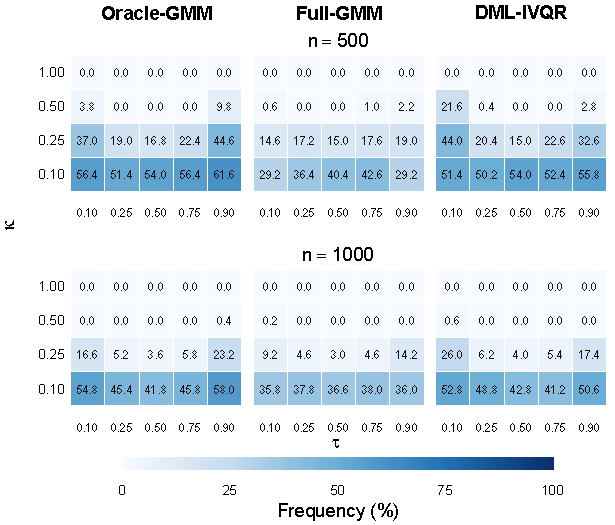
\includegraphics[width=0.72\textwidth]{figures/generated/full_domain_acceptance_heatmap.pdf}
  \caption{Full-domain grid acceptance frequencies.}
  \label{fig:appendix_full_domain_acceptance}
  \begin{figurenotes}
    Each cell reports the percentage of 500 complete replications accepting all 41 evaluated grid points in $A_0=[-1,3]$, with step size $h=0.1$. Panel columns identify estimators; panel rows show $n=500$ and $n=1000$. Within each panel, columns show quantiles $\tau$ and rows show relevance $\kappa$, declining from 1.00 to 0.10. Darker shading on the shared 0--100\% scale means more frequent full-domain grid acceptance. This event neither denotes acceptance of the entire real line nor establishes an unbounded unrestricted confidence region.
  \end{figurenotes}
\end{figure}

\FloatBarrier
\clearpage
